%!TEX root = ../../thesis.tex

\subsection{Global electroweak fit}
\label{sec:implications:ewfit}

In \Section~\ref{sec:prior_constraints:ew_fits}, a global fit of electroweak data was used 
to motivate a low mass Higgs boson. The discovery of the Higgs boson and the measurement 
of its mass enables electroweak theory to be overconstrained, and its validity can be 
tested. 

The updated fit exhibits a $p$-value of 0.176, corresponding to a deviation from the 
Standard Model of significance $1.35\sigma$ \cite{Gfitter:2013}. Thus, the experimental 
data included in the fit are consistent with electroweak theory. The pulls of individual 
fit parameters are shown in \Figure~\ref{fig:concl:ewfit_pulls}; the dominant tension is 
unrelated to \mH. The measurement of \mH does cause some tension with the measured \mW and 
$m_{\Ptop}$, though this is unsurprising since these were driving the constraint of \mH 
(through loop corrections).

\begin{figure}[p]
	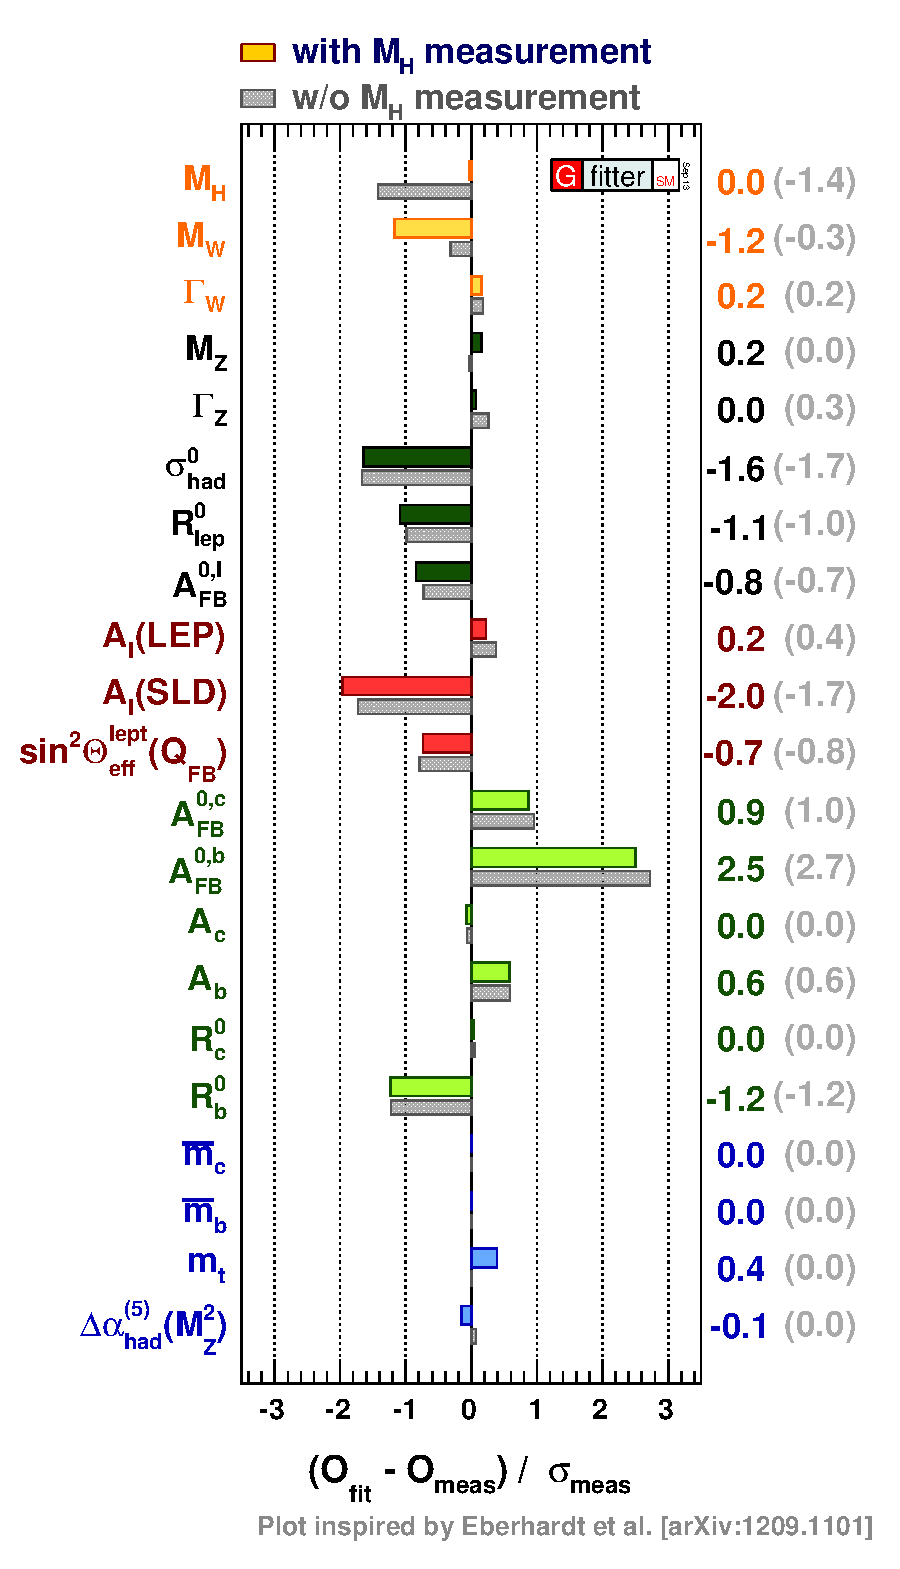
\includegraphics[width=\mediumfigwidth]{tex/conclusions/ewfit_pulls}
	\caption{Pull values of the electroweak fit parameters, with (colour) and without 
	(grey) the \mH measurement included \cite{Gfitter:2013}. The pull value is the 
	deviation of the fitted value from the experimental measurement, in units of the 
	experimental uncertainty.}
	\label{fig:concl:ewfit_pulls}
\end{figure}



\subsection{Vacuum stability}
\label{sec:implications:vacuum}

In \Section~\ref{sec:prior_constraints:theory}, theoretical arguments were used to 
constrain \mH under the assumption that the Standard Model is valid up to the reduced 
Planck scale \unit{$\bar{\Lambda}_{\text{P}}~\about~10^{18}$}{\GeV} (above which new 
physics is needed to describe gravity). Requiring the Higgs quartic coupling $\lambda$ to 
remain perturbative implied \unit{$\mH < 175$}{\GeV}, while requiring the electroweak 
vacuum to remain a stable minimum implied \unit{$\mH > 129$}{\GeV} \cite{Ellis:2009}. 

The measurement of \unit{$\mH = 126$}{\GeV} excludes the stability of the SM vacuum at 
98.6\% CL \cite{Degrassi:vacuum}. However, a potential barrier separates the vacuum in 
which the Universe currently resides and the true SM vacuum. The probability of quantum 
tunnelling through this barrier is sufficiently small that the lifetime of the Universe 
far exceeds its age. Thus, we exist in a metastable vacuum (see 
\Figure~\ref{fig:concl:vacuum_stability}).

\begin{figure}[t]
	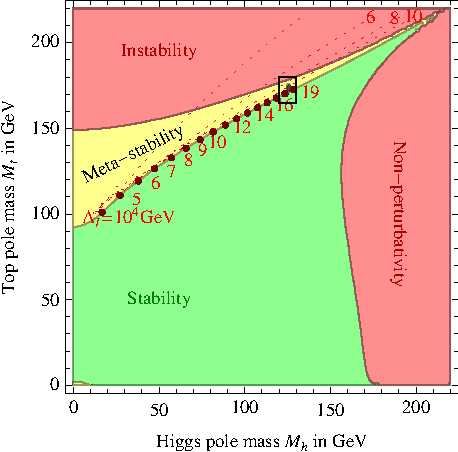
\includegraphics[width=0.48\textwidth]{tex/conclusions/vacuum_stability}
	\hfill
	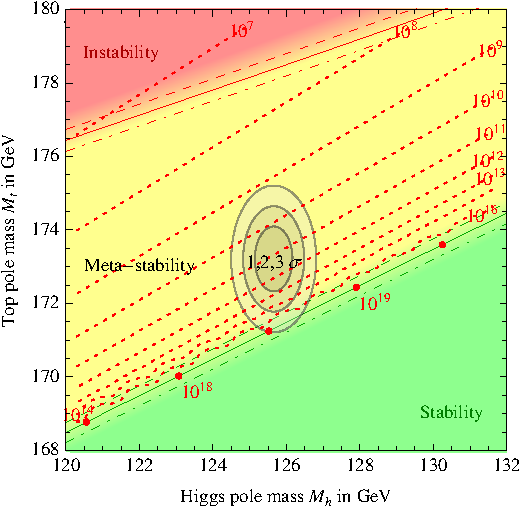
\includegraphics[width=0.49\textwidth]{tex/conclusions/vacuum_stability_zoom}
	\caption{Phase diagram of the Standard Model, expressed in terms of \mH and 
	$m_{\Ptop}$ \cite{Degrassi:vacuum}. The phases correspond to stable, metastable and 
	unstable vacuum states and a non-perturbative Higgs quartic coupling $\lambda$, 
	assuming that the scale at which new physics is introduced is 
	\unit{$\Lambda_{\text{NP}} = \Lambda_{\text{P}}~\about~10^{19}$}{\GeV}. Dotted lines 
	indicate the scale at which the instability phase transition occurs. A zoomed version 
	(right) elucidates the experimentally measured situation.}
	\label{fig:concl:vacuum_stability}
\end{figure}

The fact that experimental measurements place the Universe very close to the critical 
boundary for vacuum stability means that $\lambda$ and $\beta_{\lambda}$ are both very 
close to zero at the instability scale. Together with the scalar nature of the Higgs 
boson, this lends credence to slow-roll models of cosmic inflation with the Higgs boson 
acting as the inflaton. However, minimal configurations of such models fail to predict the 
power spectrum of anisotropies observed in the cosmic microwave background 
\cite{Isidori:2007}.



\subsection{Hierarchy problem/Naturalness}
\label{sec:implications:naturalness}


